% !Mode:: "TeX:UTF-8"
\chapter{ROS入门}
ROS是机器人研究领域一个广为探讨的主题。为了避免使本书阅读门槛太高,我们没有在正文和例程中提到它。然而近年来,ROS正逐步在各大高校的学生中间得到推广,渐渐为人们所熟知和接受,所以这里也介绍一下ROS,希望对读者能有所帮助。

\section{ROS是什么}
ROS(Robot Operating System)是Willow Garage公司于2007年发布的一个开源机器人操作系统,它为软件开发人员开发机器人应用程序提供了许多优秀的工具和库。同时,还有优秀的开发者不断地为它贡献代码。本质上,ROS并不是一个真正意义上的操作系统,而更像是基于操作系统之上的一个软件包。它提供了众多在实际机器人中可能遇到的算法:导航、通信、路径规划,等等。

ROS的版本代号是按照字母顺序来编排的,并随着Ubuntu系统发布更新。通常一个ROS版本会支持两到三个Ubuntu系统版本。ROS从Box Turtle开始,截止到本书写作时(2016年),已经更新到了Kinetic Kame(见\autoref{fig:ROS-distro})。同时,ROS也已经彻底重构,推出了实时性更强的2.0版本。

\begin{figure}[!ht]
	\centering
	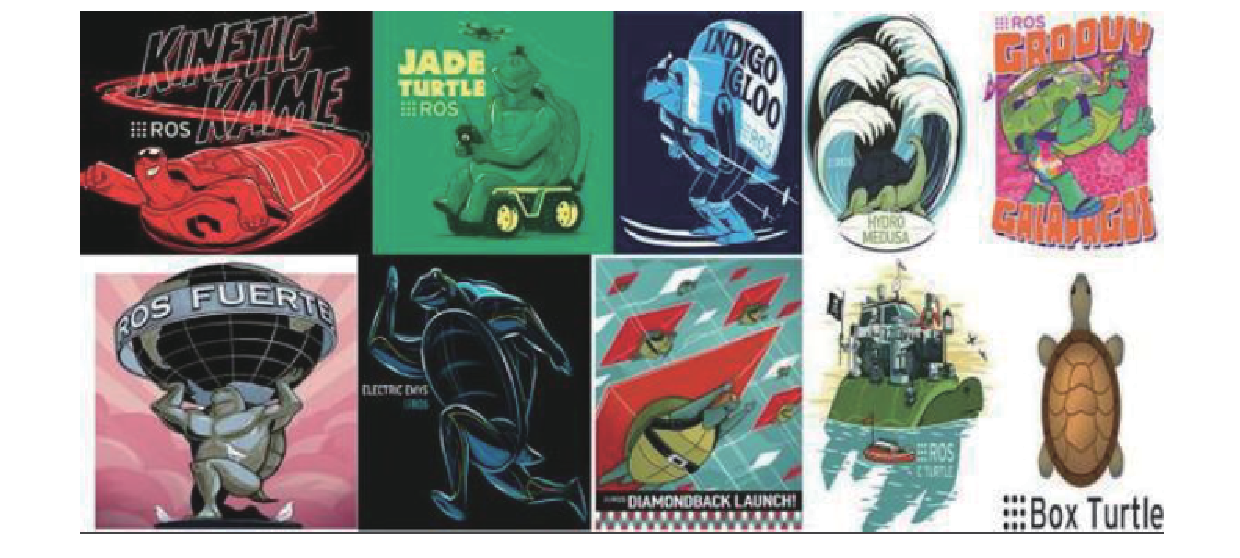
\includegraphics[width=.8\textwidth]{ROS/ROS-distro.pdf}
	\caption{ROS各版本命名方式。}
	\label{fig:ROS-distro}
\end{figure}

ROS支持很多操作系统,支持最完善的是Ubuntu及其衍生版本(Kubuntu、Linux Mint、Ubuntu GNOME等),对其他Linux发布版本、Windows等的支持也有,不过没有那么完善。因此,推荐读者使用Ubuntu操作系统来进行开发和研究。

ROS支持目前被广泛使用的面向对象的编程语言C++,以及脚本语言Python。你可以选择自己喜欢的语言进行开发。

\section{ROS的特点}
ROS的设计初衷,就是使机器人开发能够像计算机开发一样,屏蔽底层硬件及其接口的不一致性,最终使得软件可以复用。

而软件复用也正是软件工程优美性最集中的体现之一,ROS能够以统一消息格式来使得大家只需要关注算法层面的设计,而底层硬件的根本目的是接收各种各样的消息,如图像、数据等。各个硬件厂商将接收到的数据都统一到ROS所规定的统一消息格式下,即可让用户方便地使用各种开源的机器人相关算法。

在第14讲中提到的常见的开源SLAM方案中,ORB-SLAM、ORB-SLAM2、LSD-SLAM、SVO、DVO、RTAB-MAP、RGBD-SLAM-V2、Hector SLAM、Gmapping、ROVIO等均有ROS版本的开源代码,你可以很方便地在ROS中运行、调试和修改它们。

在调试SLAM程序时,数据的来源通常有3种:传感器、数据集,以及bag文件。若手头没有相应的传感器,通常就需要利用虚拟的数据来跑SLAM程序。其中,最方便的方式当属利用ROS下的bag文件发布topic,然后SLAM程序就可以监视topic发出的数据,就像使用真实的传感器采集数据一样。后面我们会简单介绍一下如何利用bag文件来模拟真实的传感器数据。

\enlargethispage{5pt}
\section{如何快速上手ROS}
ROS有完善的维基系统。因而,按照官网的介绍在机器上安装对应版本的ROS:\url{http://wiki.ros.org/ROS/Installation};然后,阅读ROS自带的教学程序即可。你会学习到ROS的基本概念、主题的发布和订阅,以及用Python和C++控制它们。如果你觉得麻烦,也可以使用针对ROS定制的Ubuntu:\url{http://www.aicrobo.com/ubuntu_for_ros.html}。

除了基本知识之外,你还可以学到一些ROS的常用工具,例如:

\begin{enumerate}
	\item rqt。rqt是ROS下的一个软件框架,它以插件的方式提供了各种各样方便好用的GUI(用户图形界面)。rqt的功能非常强大,可以实时地查看ROS中流动的消息。
	\item rosbag。rosbag是ROS提供的一个非常好用的录制及播放topic数据的工具。当你想实际跑一下SLAM程序,但囿于手头没有实际的传感器时,可以考虑使用公开提供的bag文件来进行图像或者数据的模拟,这种方式与使用一个真实的传感器在感觉上并无不同。rosbag的使用方式请参考ROS的维基页面。此外,许多公开数据集也会提供bag格式的数据文件。
	\item rviz。rviz是ROS提供的可视化模块,你可以通过它实时地查看ROS中的图像、点云、地图、规划的路径,等等,从而更方便地调试程序。
\end{enumerate}

我们相信,机器人的硬件层面和软件层面一定都会向着统一架构的方向前行,而ROS正是软件架构层面标准化一个重要的里程碑。其中,ROS 1.x在之前被大量用于实验室的研究,或者公司产品demo的研发阶段,而ROS2则解决了ROS实时性的问题,未来很有可能被直接用于实际产品的研发,为推进工业级机器人和服务机器人的应用做出重要的贡献。

本附录概述性地介绍了有关ROS的历史、优点,以及如何利用ROS中的一些可视化工具来辅助SLAM程序开发等。我们希望读者系统地学习ROS,并使用ROS开发自己的SLAM程序。